% Separado de setup-hardware.tex em 2026-11-04: as ferramentas e o módulo ficam antes
%   (ferramentas); as arquiteturas, as matrizes de teste e a potência vêm depois do formato.
\subsection{\texorpdfstring{\textcolor{red}{Hardware Architectures}}{Hardware Architectures}}\label{subsec:hw-arquiteturas}
% ---------------------------------------------------------------------
\textcolor{red}{Cada condição de teste define um intervalo máximo entre inversões, $T_c/N_{\text{PRB}}$ (Seção~\ref{subsec:restricao-vazao}). Com o clock de 100~MHz, esse intervalo é dado em ciclos. Foi feita uma arquitetura para cada condição de teste, com diretivas do HLS que reduzem o intervalo até ele atender esse limite. Também foi implementada uma versão sem otimizações de ciclos, como base de comparação. Essa versão não tem diretivas. Além disso, o Vitis HLS aplica \textit{pipeline} sozinho aos laços internos. Nessa versão, esse \textit{pipeline} automático foi desligado, com a opção \texttt{syn.compile.pipeline\_loops=0}. Assim, as iterações de cada laço rodam uma depois da outra. A Tabela~\ref{tab:hw-arquiteturas} mostra as arquiteturas.}
% ANTIGO (2026-11-06): ... como base de comparação. A Tabela~\ref{tab:hw-arquiteturas} mostra as arquiteturas.
% FONTE: hardware/cholesky_hardware/hls_config_sintese_24_12.cfg, linhas 9-10 e 16 ("pipeline_loops=0
%   desliga o pipeline automático que o Vitis aplica sozinho nos laços internos (padrão 64). Sem
%   isso a síntese já sai com 12 laços pipelinados"). TODO FONTE: guia do Vitis HLS (UG1399),
%   opção syn.compile.pipeline_loops, se a banca pedir referência do comportamento padrão.
% EN (versão anterior, 2026-11-05): Each test condition sets a maximum interval between inversions, $T_c/N_{\text{PRB}}$ (Section~\ref{subsec:restricao-vazao}). At 100~MHz, this interval is given in clock cycles. One architecture was designed for each test condition, with HLS directives that reduce the interval until it meets this limit. A version without cycle optimizations was also implemented, as a baseline. Table~\ref{tab:hw-arquiteturas} shows the architectures.

\begin{table}[htbp]
\caption{\textcolor{red}{Arquiteturas de hardware do módulo de inversão.}}
\label{tab:hw-arquiteturas}
\vspace{4pt}
\centering
\footnotesize
\color{red}% conteúdo da tabela traduzido para o português (2026-11-05); era em inglês
\renewcommand{\arraystretch}{1.2}
\begin{tabular}{lp{2.2cm}p{1.6cm}p{6.2cm}}
\toprule
\textbf{Arquitetura} & \textbf{Condição de teste alvo} & \textbf{Limite de ciclos} & \textbf{Principal otimização} \\
\midrule
Sem otimização & -- & -- & Sem diretivas; \textit{pipeline} automático de laços desligado \\
9090 & TDLA30-5 & 9.090 & Laços com \textit{pipeline} na decomposição, na substituição direta e na inversão \\
4545 & TDLA30-10 & 4.545 & A mesma, mais \textit{dataflow} entre as etapas \\
606 & TDLA30-75 & 606 & Lote de 12 matrizes em 6 vias, com \textit{dataflow} \\
455 & TDLC300-100 & 454 & Lote de 16 matrizes em 8 vias \\
152 & TDLA30-300 & 151 & Arranjo sistólico, lote de 32 matrizes em 2 vias \\
114 & TDLB100-400 & 113 & Arranjo sistólico, lote de 32 matrizes em 4 vias \\
\bottomrule
\end{tabular}
\vspace{4pt}
\legend{\textcolor{red}{Fonte: a autora. Limite de ciclos da Tabela~\ref{tab:limite-ciclos}.}}
% ANTIGO (2026-11-05): legenda "Limite de ciclos: T_c/N_PRB, com N_PRB = 275, a 100 MHz"; limites 152, 455 e 114
%   estavam arredondados para cima. Os nomes das arquiteturas (152, 455, 114) não mudaram.
% EN (versão anterior, 2026-11-05): Source: the author. Cycle limit: $T_c/N_{\text{PRB}}$ with $N_{\text{PRB}} = 275$, at 100~MHz.
\end{table}
% FONTE: acompanhamento_experimentos.csv (coluna "descrição da otimização aplicada");
%   LEIAME.md de cada pasta cholesky_hardware_diretivas*; pipeline_loops=0 em
%   hls_config_sintese_24_12*.cfg. Limites: memória tcc-constraints-tempo-estado.
% A CONFERIR: descrição da 4545 ("alterações 0 e 1 (dataflow)") e da 9090 ("alterações
%   1 a 3, 5 e 6") -- detalhar a partir dos LEIAME se a banca precisar.
% Os ciclos obtidos (7.594, 3.020, 504, 402, 128, 64 em <24,12>) são RESULTADO: vão para
%   os Resultados, com a origem (log xsim do servidor), e mudam com o formato.

\textcolor{red}{As arquiteturas otimizadas foram implementadas só em $16 \times 16$. Em $32 \times 32$, só a versão sem otimizações foi implementada no Vivado.}
% EN (versão anterior, 2026-11-05): The optimized architectures were implemented only in $16 \times 16$. In $32 \times 32$, only the version without optimizations was implemented in Vivado.
% FONTE: acompanhamento_experimentos.csv, linha "otimizações de ciclos (32 x 32)":
%   só síntese C local; nenhuma atende o alvo de ciclos; 114 não cabe. Isso é resultado:
%   a frase aqui só diz o que foi implementado; o porquê vai para os Resultados.

\textcolor{red}{Todas as arquiteturas calculam a mesma inversa que a versão sem otimizações. Isso foi conferido bit a bit, com o código C de cada versão, nos formatos escolhidos e nos dois tamanhos de matriz.}
% EN (versão anterior, 2026-11-05): Every architecture computes the same inverse as the version without optimizations. This was checked bit by bit, with the C code of each version, in the chosen formats and in both matrix sizes.
% FONTE: comparar_com_original.py (LEIAME de cada versão); conferir_formatos_novos.sh
%   para <26,12> e <30,14> (iguais nas 6 arquiteturas, 16x16 e 32x32).

% =====================================================================
% Subseções das otimizações (2026-11-06). Uma por tipo de otimização, com figura,
%   diretiva e trecho de código. Fontes: Kastner (books/Parallel Programming for
%   FPGAs.pdf) e o código de cada pasta hardware/cholesky_hardware_diretivas*.
% As figuras são esquemáticas: nenhum número medido aqui (os ciclos medidos são
%   resultado e vão para os Resultados). Os trechos de código são simplificados.
% =====================================================================
\subsubsection{\texorpdfstring{\textcolor{red}{Pipeline e tempo de enchimento}}{Pipeline e tempo de enchimento}}\label{subsubsec:hw-pipeline}

\textcolor{red}{Todas as arquiteturas otimizadas usam \textit{pipeline}. Sem \textit{pipeline}, as iterações de um laço rodam uma depois da outra \cite[p.~43]{kastner-hls}. Com \textit{pipeline}, uma iteração começa antes de a anterior terminar \cite[p.~45]{kastner-hls}. No começo, o \textit{pipeline} está vazio, e só os primeiros estágios trabalham. O tempo até todos os estágios ficarem ocupados é o tempo de enchimento do \textit{pipeline}. Depois dele, todos os estágios trabalham ao mesmo tempo, cada um com um dado diferente \cite[p.~114]{kastner-hls}.}
% ANTIGO (2026-11-06): depois do cite p. 43, "Na versão sem otimizações, o pipeline automático de
%   laços foi desligado (Tabela tab:hw-arquiteturas)." Foi para o primeiro parágrafo da subseção.
% Definição do enchimento: redação própria. O livro do Kastner não tem uma frase literal
%   sobre "pipeline fill" ou "startup". As passagens mais próximas: p. 114 ("Once the
%   pipeline is full, all four subfunctions are executing concurrently, but each one is
%   operating on different input data"), p. 45 (exemplo abaixo) e p. 146 (esvaziamento).

\textcolor{red}{No exemplo do livro, cada iteração de um laço leva 4 ciclos, e o laço tem 11 iterações, com II de 1 ciclo. A primeira iteração termina no ciclo 4, e a última, no ciclo 14 \cite[p.~45]{kastner-hls}. Ou seja, o laço leva $4 + (11-1) \cdot 1 = 14$ ciclos. No fim do laço, o \textit{pipeline} precisa esvaziar antes de o código seguinte começar. Por isso, a profundidade do \textit{pipeline} é um custo fixo, que pesa mais quando o laço tem poucas iterações \cite[p.~146]{kastner-hls}.}

\textcolor{red}{O mesmo vale para tarefas inteiras, como a inversão de uma matriz. Seja $L$ a latência de uma tarefa e $I$ o intervalo em regime (Seção~\ref{subsubsec:latencia-intervalo}). A primeira tarefa termina depois de $L$, e cada tarefa seguinte termina $I$ depois da anterior. Assim, $n$ tarefas seguidas terminam em}
\begin{equation}\label{eq:fim-tarefas}
\textcolor{red}{t_n = L + (n-1)\, I.}
\end{equation}
\textcolor{red}{O limite de ciclos da Tabela~\ref{tab:limite-ciclos} vale para o intervalo $I$, e não para a latência $L$. As subseções a seguir mostram como cada otimização reduz o intervalo.}

% ---------------------------------------------------------------------
\subsubsection{\texorpdfstring{\textcolor{red}{Pipeline de laços}}{Pipeline de laços}}\label{subsubsec:hw-pipeline-lacos}

\textcolor{red}{A arquitetura 9090 coloca a diretiva \texttt{\#pragma HLS pipeline II=1} nos laços internos das etapas do módulo (Figura~\ref{fig:modulo-inversao}). Só a etapa \texttt{D\_extraction} fica sem a diretiva. Essa diretiva pede ao HLS um II de 1 ciclo. Se as dependências ou os recursos não permitirem, o HLS usa um II maior \cite[p.~45]{kastner-hls}.}
% FONTE: cholesky_hardware_diretivas/{lu_decomposition, foward_substitution, inversion,
%   g_step, s_step}.cpp (pipeline II=1 nos laços internos); dv_step.cpp (D_extraction) sem pragma.

\textcolor{red}{A Figura~\ref{fig:hw-pipeline-lacos} mostra um laço da decomposição LU. Sem \textit{pipeline}, cada iteração espera a anterior terminar. Com II = 1, uma iteração nova começa a cada ciclo. Os quatro estágios só ficam ocupados no ciclo 4, quando a primeira iteração termina. Assim, o enchimento dura cerca de uma latência de iteração. O esvaziamento, no fim do laço, também. As etapas e os laços de uma matriz ainda rodam um depois do outro. Assim, a próxima inversão só começa depois que a anterior termina \cite[p.~114]{kastner-hls}. Nessa arquitetura, o intervalo entre inversões é igual à latência de uma inversão.}

\begin{figure}[!ht]
\caption{\textcolor{red}{Loop pipelining in the LU decomposition. The code is simplified.}}
\label{fig:hw-pipeline-lacos}
\vspace{4pt} % a classe zera o espaço entre a caption e a figura
\centering
\begin{minipage}[c]{0.40\textwidth}
\color{red}\fontsize{7}{8.6}\selectfont
\begin{verbatim}
for (line = column + 1; line < n; line++)
  for (k = column; k < n; k++) {
#pragma HLS pipeline II=1
    t = L[line][column] * U[column][k];
    U[line][k] = U[line][k] - t;
  }
\end{verbatim}
\end{minipage}\hfill
\begin{minipage}[c]{0.57\textwidth}
\centering
\begin{tikzpicture}[font=\fontsize{6.5}{7.8}\selectfont,
  every node/.append style={text=red},
  est/.style={draw=black!60, fill=#1, minimum width=0.50cm, minimum height=0.32cm, inner sep=0pt, line width=0.3pt},
  est/.default=white]
\def\u{0.50}\def\h{0.38}
\definecolor{e1}{HTML}{CDE2FB}\definecolor{e2}{HTML}{9EC5F4}\definecolor{e3}{HTML}{6FA6E8}\definecolor{e4}{HTML}{D9D9D9}
% estágios de uma iteração: Rd, Mul, Sub, Wr (latência de 4 ciclos)
\newcommand{\iter}[3]{% #1 = ciclo de início (0-index), #2 = linha, #3 = rótulo
  \node[est=e1] at (#1*\u+0.5*\u, -#2*\h) {\fontsize{5}{6}\selectfont Rd};
  \node[est=e2] at (#1*\u+1.5*\u, -#2*\h) {\fontsize{5}{6}\selectfont Mul};
  \node[est=e3] at (#1*\u+2.5*\u, -#2*\h) {\fontsize{5}{6}\selectfont Sub};
  \node[est=e4] at (#1*\u+3.5*\u, -#2*\h) {\fontsize{5}{6}\selectfont Wr};
  \node[left] at (-0.05, -#2*\h) {#3};}
% (a) sem pipeline
\node[anchor=west] at (-1.0, 0.62) {(a) Without pipeline};
\iter{0}{0}{it.~1}
\begin{scope}[shift={(4*\u,0)}]
  \node[est=e1] at (0.5*\u,0) {\fontsize{5}{6}\selectfont Rd};
  \node[est=e2] at (1.5*\u,0) {\fontsize{5}{6}\selectfont Mul};
  \node[est=e3] at (2.5*\u,0) {\fontsize{5}{6}\selectfont Sub};
  \node[est=e4] at (3.5*\u,0) {\fontsize{5}{6}\selectfont Wr};
\end{scope}
\node at (6*\u, 0.30) {it.~2};
\node[right] at (8*\u, 0) {$\cdots$ next iteration after 4 cycles};
% (b) com pipeline, II = 1, 6 iterações
\begin{scope}[shift={(0,-1.30)}]
\node[anchor=west] at (-1.0, 0.62) {(b) Pipeline, II = 1};
\foreach \i in {0,...,5} { \pgfmathtruncatemacro{\r}{\i+1} \iter{\i}{\i}{it.~\r} }
% eixo dos ciclos
\foreach \c in {1,...,9} \node[text=red!70!black] at (\c*\u-0.5*\u, -6*\h+0.02) {\fontsize{5}{6}\selectfont\c};
\node[left] at (-0.05, -6*\h+0.02) {cycle};
% II
\draw[red, |<->|, line width=0.4pt] (0,0.24) -- (\u,0.24) node[midway, above=-1pt] {II};
% enchimento, regime e esvaziamento
\draw[decorate, decoration={brace, mirror, amplitude=3pt}, red, line width=0.4pt] (0.02,-6*\h-0.15) -- (3*\u-0.02,-6*\h-0.15) node[midway, below=2pt, align=center] {fill};
\draw[decorate, decoration={brace, mirror, amplitude=3pt}, red, line width=0.4pt] (3*\u+0.02,-6*\h-0.15) -- (6*\u-0.02,-6*\h-0.15) node[midway, below=2pt, align=center] {full};
\draw[decorate, decoration={brace, mirror, amplitude=3pt}, red, line width=0.4pt] (6*\u+0.02,-6*\h-0.15) -- (9*\u-0.02,-6*\h-0.15) node[midway, below=2pt, align=center] {flush};
\draw[decorate, decoration={brace, amplitude=3pt}, red, line width=0.4pt] (9*\u+0.12,0.15) -- (9*\u+0.12,-5*\h-0.15) node[midway, right=3pt, align=left] {loop latency\\$4 + (6-1)\cdot 1 = 9$};
\end{scope}
\end{tikzpicture}
\end{minipage}
\vspace{4pt}
\legend{\textcolor{red}{Source: the author. Rd: read, Mul: multiply, Sub: subtract, Wr: write. Iteration latency of 4 cycles, as in the example of the book \cite[p.~45]{kastner-hls}.}}
\end{figure}

% ---------------------------------------------------------------------
\subsubsection{\texorpdfstring{\textcolor{red}{Dataflow entre etapas}}{Dataflow entre etapas}}\label{subsubsec:hw-dataflow}

\textcolor{red}{A arquitetura 4545 mantém o \textit{pipeline} dos laços e junta as funções do módulo em quatro etapas. A primeira é a decomposição LU. A segunda calcula a matriz $\mathbf F$ (\texttt{D\_extraction}, \texttt{D\_square\_root} e \texttt{G\_decomposition}). A terceira é a substituição direta, e a quarta, a inversão. A diretiva \texttt{\#pragma HLS dataflow}, na função de topo, transforma cada etapa em um processo. Assim, uma matriz nova entra na primeira etapa assim que a matriz anterior passa para a segunda \cite[p.~114]{kastner-hls}.}
% FONTE: cholesky_hardware_diretivas_4545/cholesky_top.cpp (etapa_lu, etapa_g, etapa_fs,
%   etapa_inv; dataflow em cholesky_inverse, linha 68).

\textcolor{red}{O \textit{dataflow} forma um \textit{pipeline} de tarefas, controlado pela troca de sinais entre os processos. O \textit{pipeline} de laços, por sua vez, age ciclo a ciclo \cite[pp.~114--115]{kastner-hls}. Entre dois processos, os dados passam por uma FIFO ou por um \textit{buffer} ping-pong. O \textit{buffer} ping-pong tem dois blocos: o processo que produz os dados escreve em um, enquanto o processo que os consome lê o outro \cite[p.~115]{kastner-hls}.}

\textcolor{red}{Cada etapa leva a diretiva \texttt{\#pragma HLS inline off}. Essa diretiva impede o HLS de copiar a função para dentro da função que a chama, e mantém a hierarquia do código \cite[p.~52]{kastner-hls}. Assim, cada etapa continua sendo uma função separada e vira um processo.}

\textcolor{red}{Na Figura~\ref{fig:hw-dataflow}, a latência de uma matriz é a soma das quatro etapas. Uma etapa só recebe a matriz seguinte depois de terminar a anterior. Por isso, o intervalo é a duração da etapa mais longa. Sem \textit{dataflow}, a matriz 2 só começaria no fim da matriz 1.}
% SEM FONTE: "intervalo = etapa mais longa" é lido da figura (não achei frase no Kastner;
%   a p. 97 fala de "weakest link", mas de uma porta de memória).

\begin{figure}[!ht]
\caption{\textcolor{red}{Dataflow between the stages of the inversion. The code is simplified, and the durations are not to scale.}}
\label{fig:hw-dataflow}
\vspace{4pt}
\centering
\begin{minipage}[c]{0.33\textwidth}
\color{red}\fontsize{7}{8.6}\selectfont
\begin{verbatim}
void cholesky_inverse(A, inverse) {
#pragma HLS dataflow
  etapa_lu(A, L, U);
  etapa_g(U, L, G);
  etapa_fs(G, G_inv);
  etapa_inv(G_inv, inverse);
}

static void etapa_fs(G, G_inv) {
#pragma HLS inline off
  forward_substitution(G, G_inv);
}
\end{verbatim}
\end{minipage}\hfill
\begin{minipage}[c]{0.64\textwidth}
\centering
\begin{tikzpicture}[font=\fontsize{6.5}{7.8}\selectfont,
  every node/.append style={text=red},
  tar/.style={draw=black!60, fill=#1, minimum height=0.34cm, inner sep=0pt, line width=0.3pt}]
\def\u{0.40}\def\h{0.46}
\definecolor{m1}{HTML}{CDE2FB}\definecolor{m2}{HTML}{9EC5F4}\definecolor{m3}{HTML}{D9D9D9}
% durações esquemáticas: LU = 4, G = 1, FS = 2, INV = 2 (soma 9, maior 4)
\newcommand{\caixa}[5]{% #1 linha, #2 início, #3 duração, #4 cor, #5 matriz
  \node[tar=#4, minimum width=#3*\u cm, anchor=west] at (#2*\u, -#1*\h) {#5};}
\foreach \l/\n in {0/etapa\_lu, 1/etapa\_g, 2/etapa\_fs, 3/etapa\_inv}
  \node[left, font=\fontsize{6.2}{7.4}\selectfont\ttfamily] at (-0.05, -\l*\h) {\n};
% matriz 1
\caixa{0}{0}{4}{m1}{1}\caixa{1}{4}{1}{m1}{1}\caixa{2}{5}{2}{m1}{1}\caixa{3}{7}{2}{m1}{1}
% matriz 2
\caixa{0}{4}{4}{m2}{2}\caixa{1}{8}{1}{m2}{2}\caixa{2}{9}{2}{m2}{2}\caixa{3}{11}{2}{m2}{2}
% matriz 3
\caixa{0}{8}{4}{m3}{3}\caixa{1}{12}{1}{m3}{3}\caixa{2}{13}{2}{m3}{3}\caixa{3}{15}{2}{m3}{3}
% eixo
\draw[black!60, ->, line width=0.4pt] (0,-3*\h-0.3) -- (17.6*\u,-3*\h-0.3) node[right] {time};
% intervalo
\draw[red, |<->|, line width=0.4pt] (0,0.30) -- (4*\u,0.30) node[midway, above=-1pt] {interval $I$ = longest stage};
% latência da matriz 1
\draw[red, |<->|, line width=0.4pt] (0,-3*\h-0.55) -- (9*\u,-3*\h-0.55) node[midway, below=-1pt] {latency $L$ = sum of the stages};
% sem dataflow
\draw[red, dashed, line width=0.4pt] (9*\u,0.18) -- (9*\u,-3*\h-0.3);
\node[align=left, anchor=south west] at (9*\u+0.05,0.05) {without dataflow,\\matrix 2 starts here};
% fim da matriz 3
\draw[red, |<->|, line width=0.4pt] (0,-3*\h-1.0) -- (17*\u,-3*\h-1.0) node[midway, below=-1pt] {matrix 3 ends at $L + 2I$ (Equation~\ref{eq:fim-tarefas})};
\end{tikzpicture}
\end{minipage}
\vspace{4pt}
\legend{\textcolor{red}{Source: the author. Numbers in the boxes: index of the matrix.}}
\end{figure}

% ---------------------------------------------------------------------
\subsubsection{\texorpdfstring{\textcolor{red}{Lotes de matrizes em vias}}{Lotes de matrizes em vias}}\label{subsubsec:hw-lotes}

\textcolor{red}{Nas arquiteturas 606 e 455, o módulo recebe várias matrizes $\mathbf G_c$ de uma vez, cada uma de um PRB. Esse conjunto é um lote. O lote tem 12 matrizes na 606 e 16 na 455. As matrizes de um lote não dependem umas das outras. As etapas do lote formam um \textit{dataflow}, como na 4545, e um lote novo entra a cada intervalo de lote. O intervalo por matriz é o intervalo do lote dividido pelo número de matrizes do lote, e é ele que deve atender o limite da Tabela~\ref{tab:limite-ciclos}. O número de lotes de um bloco é $N_{\text{PRB}}$ dividido pelo tamanho do lote, arredondado para cima. O último lote vai incompleto. Na Equação~\eqref{eq:fim-tarefas}, a tarefa passa a ser o lote.}
% FONTE: cholesky_hardware_diretivas_606/cholesky_top.cpp (comentário do topo; LOTE e
%   VIAS em cholesky.h; dataflow na linha 315 com lote_ler, lote_lu, lote_g, lote_fs,
%   lote_inv, lote_gravar). LOTE/VIAS: 12/6 (606), 16/8 (455).

\textcolor{red}{As matrizes do lote ficam em bancos de memória separados, com a diretiva \texttt{\#pragma HLS array\_partition cyclic} no índice da matriz. A partição cíclica distribui os elementos entre os bancos de forma alternada. Por exemplo, com fator 2, o vetor 1, 2, \ldots, 9 vira os vetores 1, 3, 5, 7, 9 e 2, 4, 6, 8 \cite[p.~88]{kastner-hls}. Com fator igual ao número de vias, a matriz $m$ fica no banco $m \bmod \text{vias}$. Uma via é o conjunto de operadores que trata um banco. A 606 tem 6 vias, e a 455, 8.}

\textcolor{red}{A Figura~\ref{fig:hw-lotes} mostra a 606. Em cada ciclo, o laço com \textit{pipeline} faz a mesma conta em 6 matrizes, uma em cada via. O lote é tratado em grupos de 6 matrizes, que se alternam a cada ciclo. Como as matrizes não dependem umas das outras, uma iteração não espera o resultado da anterior. As divisões também alternam entre as matrizes do lote, uma por ciclo. Assim, o divisor, que tem \textit{pipeline}, não espera o resultado da divisão anterior.}

\begin{figure}[!ht]
\caption{\textcolor{red}{Batch of 12 matrices in 6 lanes, in the 606 architecture. The code is simplified.}}
\label{fig:hw-lotes}
\vspace{4pt}
\centering
\begin{minipage}[c]{0.43\textwidth}
\color{red}\fontsize{7}{8.6}\selectfont
\begin{verbatim}
#pragma HLS array_partition variable=U \
                     cyclic factor=VIAS dim=1
for (k = column; k < n; k++)
  for (g = 0; g < GRUPOS; g++) {
#pragma HLS pipeline II=1
    for (p = 0; p < VIAS; p++) {
      m = g * VIAS + p;
      t = L[m][line][column] * U[m][column][k];
      U[m][line][k] = U[m][line][k] - t;
    }
  }
\end{verbatim}
\end{minipage}\hfill
\begin{minipage}[c]{0.54\textwidth}
\centering
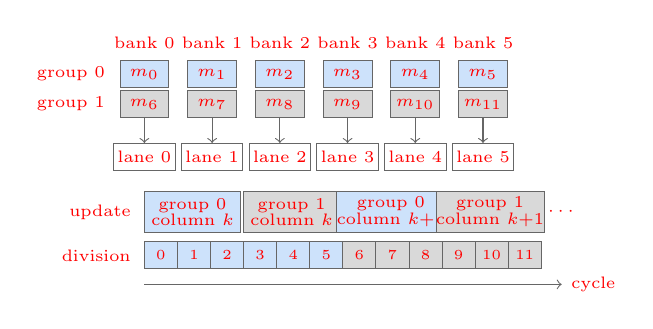
\begin{tikzpicture}[font=\fontsize{6.5}{7.8}\selectfont,
  every node/.append style={text=red},
  mat/.style={draw=black!60, fill=#1, minimum width=0.62cm, minimum height=0.34cm, inner sep=0pt, line width=0.3pt},
  via/.style={draw=black!60, fill=white, minimum width=0.78cm, minimum height=0.34cm, inner sep=0pt, line width=0.3pt}]
\def\u{0.86}
\definecolor{g0}{HTML}{CDE2FB}\definecolor{g1}{HTML}{D9D9D9}
% bancos: matriz m no banco m mod 6
\foreach \p in {0,...,5} {
  \pgfmathtruncatemacro{\q}{\p+6}
  \node at (\p*\u, 0.40) {bank \p};
  \node[mat=g0] at (\p*\u, 0) {$m_{\p}$};
  \node[mat=g1] at (\p*\u, -0.38) {$m_{\q}$};
  \node[via] (v\p) at (\p*\u, -1.05) {lane \p};
  \draw[black!60, ->, line width=0.4pt] (\p*\u, -0.56) -- (v\p.north);
}
\node[left] at (-0.38, 0) {group 0};
\node[left] at (-0.38, -0.38) {group 1};
% ciclos do laço de atualização
\begin{scope}[shift={(0,-1.75)}]
\foreach \c/\g/\k/\cor in {0/0/k/g0, 1/1/k/g1, 2/0/k{+}1/g0, 3/1/k{+}1/g1} {
  \node[mat=\cor, minimum width=1.22cm, minimum height=0.52cm, align=center, font=\fontsize{6}{7}\selectfont] at (\c*1.26+0.61, 0) {group \g\\[-1pt]column $\k$};
}
\node[left] at (-0.05, 0) {update};
\node[right] at (5.0, 0) {$\cdots$};
\foreach \c in {0,...,11} {
  \pgfmathtruncatemacro{\gg}{\c<6 ? 0 : 1}
  \ifnum\gg=0 \def\cc{g0}\else\def\cc{g1}\fi
  \node[mat=\cc, minimum width=0.42cm] at (\c*0.42+0.21, -0.55) {\fontsize{5.5}{6}\selectfont\c};
}
\node[left] at (-0.05, -0.55) {division};
\draw[black!60, ->, line width=0.4pt] (0,-0.92) -- (5.3,-0.92) node[right] {cycle};
\end{scope}
\end{tikzpicture}
\end{minipage}
\vspace{4pt}
\legend{\textcolor{red}{Source: the author. Update: one cycle per box, 6 matrices at a time. Division: one matrix per cycle, in a single divider; the numbers are the indices $m$ of the matrices.}}
\end{figure}

% ---------------------------------------------------------------------
\subsubsection{\texorpdfstring{\textcolor{red}{Arranjo sistólico}}{Arranjo sistólico}}\label{subsubsec:hw-sistolico}

\textcolor{red}{As arquiteturas 152 e 114 também usam lotes, com 32 matrizes. A 152 tem 2 vias, e a 114 tem 4. Cada via tem o seu próprio divisor. Além disso, o laço que percorre uma linha ou uma soma é desenrolado em células, uma para cada índice $k$, lado a lado. Cada célula só troca dados com a vizinha. Projetos assim são chamados de arranjos sistólicos, e podem surgir quando um laço interno é desenrolado \cite[p.~180]{kastner-hls}.}
% FONTE: cholesky_hardware_diretivas_152_sistolico/cholesky_top.cpp (comentário do topo);
%   LOTE/VIAS: 32/2 (152), 32/4 (114).

\textcolor{red}{Na substituição direta e na inversão, a soma parcial passa de uma célula para a seguinte, na mesma ordem de somas da versão sem otimizações. Assim, cada ciclo calcula uma soma inteira. Na decomposição LU, cada célula atualiza um elemento da linha, e cada ciclo atualiza uma linha inteira. Para as células lerem todos os índices $k$ no mesmo ciclo, cada elemento da linha fica em um banco próprio, com \texttt{\#pragma HLS array\_partition complete} \cite[p.~41]{kastner-hls}.}

\textcolor{red}{Na decomposição LU e na substituição direta, cada passo usa as linhas gravadas no passo anterior. As matrizes do lote se alternam a cada ciclo. Assim, entre a gravação de uma linha e a sua leitura, passam tantos ciclos quanto o tamanho do passo. Os passos curtos recebem ciclos vazios, até um número mínimo de ciclos. Com isso, uma linha só é lida depois de sair do \textit{pipeline}. A diretiva \texttt{\#pragma HLS dependence ... dependent=false} informa isso ao HLS. Essa diretiva passa ao HLS uma informação que ele não consegue deduzir do código, e cabe ao projetista garantir que ela é verdadeira \cite[pp.~149--150]{kastner-hls}. Se o \textit{pipeline} ficar mais profundo que o passo, o resultado fica errado. A simulação da netlist, que compara as inversas com as do código C (Seção~\ref{subsec:hw-potencia}), confere isso. A Figura~\ref{fig:hw-sistolico} mostra as células e os ciclos vazios.}
% FONTE: comentário do topo de cholesky_top.cpp da 152 (CHOL_PROF_LU, CHOL_PROF_FS;
%   lu_passo, fs_passo; "Se a profundidade real do pipeline passar de CHOL_PROF_*, o
%   resultado do RTL fica errado; a co-simulação confere isso").

\begin{figure}[!ht]
\caption{\textcolor{red}{Systolic array of the forward substitution and minimum step of the LU decomposition. The code is simplified.}}
\label{fig:hw-sistolico}
\vspace{4pt}
\centering
\begin{minipage}[c]{0.42\textwidth}
\color{red}\fontsize{7}{8.6}\selectfont
\begin{verbatim}
#pragma HLS array_partition variable=Ua \
                     complete dim=3
for (it = 0; it < LU_ITER; it++) {
#pragma HLS pipeline II=1
#pragma HLS dependence variable=Ua \
          type=inter dependent=false
  if (idx < reais)       // else: empty
    for (p = 0; p < VIAS; p++)
      for (k = 0; k < n; k++)  // cells
        Ua[m][line][k] = row[k] - l*piv[k];
}
\end{verbatim}
\end{minipage}\hfill
\begin{minipage}[c]{0.55\textwidth}
\centering
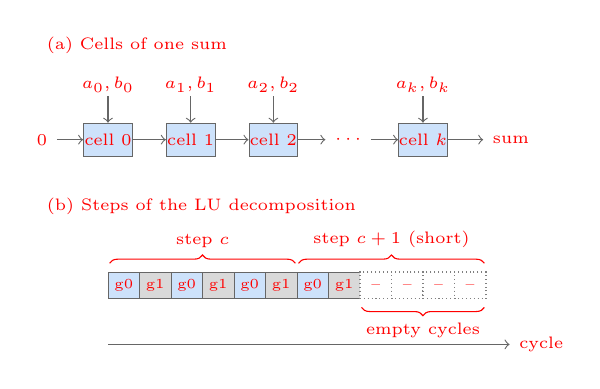
\begin{tikzpicture}[font=\fontsize{6.5}{7.8}\selectfont,
  every node/.append style={text=red},
  cel/.style={draw=black!60, fill=#1, minimum width=0.62cm, minimum height=0.42cm, inner sep=0pt, line width=0.3pt},
  cel/.default={white},
  seta/.style={black!60, ->, line width=0.4pt}]
\definecolor{c0}{HTML}{CDE2FB}\definecolor{c1}{HTML}{D9D9D9}
% (a) células em cadeia: s_k = s_{k-1} + a_k b_k
\node[anchor=west] at (-0.9, 1.20) {(a) Cells of one sum};
\foreach \k/\x/\l in {0/0/0, 1/1.05/1, 2/2.10/2} {
  \node[cel=c0] (c\k) at (\x, 0) {cell \l};
  \draw[seta] (\x, 0.55) node[above=-2pt] {$a_{\l}, b_{\l}$} -- (c\k.north);
}
\node (dots) at (3.05, 0) {$\cdots$};
\node[cel=c0] (cn) at (4.0, 0) {cell $k$};
\draw[seta] (4.0, 0.55) node[above=-2pt] {$a_{k}, b_{k}$} -- (cn.north);
\draw[seta] (-0.65, 0) node[left] {$0$} -- (c0.west);
\draw[seta] (c0) -- (c1); \draw[seta] (c1) -- (c2); \draw[seta] (c2) -- (dots); \draw[seta] (dots) -- (cn);
\draw[seta] (cn.east) -- ++(0.45, 0) node[right] {sum};
% (b) passos da LU com ciclos vazios
\begin{scope}[shift={(0,-1.85)}]
\node[anchor=west] at (-0.9, 1.00) {(b) Steps of the LU decomposition};
\def\w{0.40}
\foreach \i/\g in {0/0, 1/1, 2/0, 3/1, 4/0, 5/1} {
  \ifnum\g=0 \def\cc{c0}\else\def\cc{c1}\fi
  \node[cel=\cc, minimum width=0.40cm, minimum height=0.34cm] at (\i*\w+0.5*\w, 0) {\fontsize{5}{6}\selectfont g\g};
}
\foreach \i/\g in {6/0, 7/1} {
  \ifnum\g=0 \def\cc{c0}\else\def\cc{c1}\fi
  \node[cel=\cc, minimum width=0.40cm, minimum height=0.34cm] at (\i*\w+0.5*\w, 0) {\fontsize{5}{6}\selectfont g\g};
}
\foreach \i in {8,...,11}
  \node[draw=black!50, fill=white, densely dotted, minimum width=0.40cm, minimum height=0.34cm, inner sep=0pt, line width=0.4pt] at (\i*\w+0.5*\w, 0) {\fontsize{5}{6}\selectfont --};
\draw[decorate, decoration={brace, amplitude=3pt}, red, line width=0.4pt] (0.02, 0.28) -- (6*\w-0.02, 0.28) node[midway, above=2pt] {step $c$};
\draw[decorate, decoration={brace, amplitude=3pt}, red, line width=0.4pt] (6*\w+0.02, 0.28) -- (12*\w-0.02, 0.28) node[midway, above=2pt] {step $c+1$ (short)};
\draw[decorate, decoration={brace, mirror, amplitude=3pt}, red, line width=0.4pt] (8*\w+0.02, -0.28) -- (12*\w-0.02, -0.28) node[midway, below=2pt] {empty cycles};
\draw[black!60, ->, line width=0.4pt] (0,-0.75) -- (12*\w+0.3,-0.75) node[right] {cycle};
\end{scope}
\end{tikzpicture}
\end{minipage}
\vspace{4pt}
\legend{\textcolor{red}{Source: the author. g0 and g1: groups of matrices of the batch, one per cycle. Two groups are drawn for clarity: the 152 has 16 groups, and the 114 has 8. In (b), the short step is filled with empty cycles up to a minimum length, so that a row is read only after it leaves the pipeline.}}
\end{figure}

% ---------------------------------------------------------------------
\subsection{\texorpdfstring{\textcolor{red}{Test Matrices}}{Test Matrices}}\label{subsec:hw-matrizes}
% ---------------------------------------------------------------------
\textcolor{red}{O hardware foi testado com as matrizes $\mathbf{G}_c$ que o BCD-MMSE inverte no simulador. Um script roda o simulador com a mesma semente e salva cada $\mathbf{G}_c$ antes da inversão. O simulador não muda. Assim, as matrizes são exatamente as usadas nas curvas de SER, com 1 iteração do BCD-MMSE.}
% EN (versão anterior, 2026-11-05): The hardware was tested with the matrices $\mathbf{G}_c$ that the BCD-MMSE inverts in the simulator. A script runs the simulator with the same seed and saves each $\mathbf{G}_c$ before the inversion. The simulator does not change. So the matrices are exactly the ones used for the SER curves, with 1 BCD-MMSE iteration.
% FONTE: AMOSTRAGEM.md, seções 1 e 2 (exportar_matrizes.py troca a função de inversão
%   só na memória do processo; matrizes recalculadas por fora coincidem até 1e-12).

\textcolor{red}{Como as condições de teste só mudam $N$ e a portadora (Seção~\ref{subsec:setup_condicoes}), as matrizes foram exportadas uma vez para cada par da Tabela~\ref{tab:condicoes_teste}. São 5 pares, pois TDLA30-5 e TDLA30-10 têm o mesmo par.}
% ANTIGO (2026-11-05, repetia Test Conditions e a Tabela tab:condicoes_teste):
% \textcolor{red}{As condições de teste mudam só dois valores nessas matrizes: o número de amostras de ruído $N$ e a frequência de portadora. Condições com o mesmo $N$ e a mesma portadora dão as mesmas matrizes. Por isso, as matrizes foram exportadas uma vez para cada par: 192 amostras a 3,5~GHz (TDLA30-5 e TDLA30-10), 192 a 28~GHz (TDLA30-75), 168 a 28~GHz (TDLA30-300), 132 a 3,5~GHz (TDLC300-100) e 24 a 3,5~GHz (TDLB100-400).}
% EN (versão anterior, 2026-11-05): The test conditions change only two values in these matrices: the number of noise samples $N$ and the carrier frequency. Test conditions with the same $N$ and the same carrier give the same matrices. So the matrices were exported once for each pair: 192 samples at 3.5~GHz (TDLA30-5 and TDLA30-10), 192 at 28~GHz (TDLA30-75), 168 at 28~GHz (TDLA30-300), 132 at 3.5~GHz (TDLC300-100) and 24 at 3.5~GHz (TDLB100-400).
% FONTE: AMOSTRAGEM.md, tabela das pastas (2_amostra_matrizes/amostras<N>_fc<GHz>GHz).

\textcolor{red}{A modulação não muda $\mathbf{G}_c = E_s\mathbf{H}_c\mathbf{H}_c^H + \hat{\mathbf{R}}_{cc}$. Em cada grupo, as configurações QPSK (C, D, G e H) diferem das configurações 16-QAM (A, B, E e F) só na modulação. Por isso, as configurações QPSK não foram exportadas.}
% ANTIGO (2026-11-06): "As configurações 1C, 1D, 1G e 1H diferem de 1A, 1B, 1E e 1F só na modulação."
%   Citava só o grupo 1, mas as QPSK dos grupos 2 e 3 também não foram exportadas
%   (indice.csv: 16x16 só 1A, 1B, 1E, 1F, 3A, 3B, 3E, 3F; 32x32 só 2A, 2B, 2E, 2F).
% EN (versão anterior, 2026-11-05): The modulation does not change $\mathbf{G}_c = E_s\mathbf{H}_c\mathbf{H}_c^H + \hat{\mathbf{R}}_{cc}$. Configurations 1C, 1D, 1G and 1H differ from 1A, 1B, 1E and 1F only in the modulation. Therefore, the QPSK configurations were not exported.
% FONTE: AMOSTRAGEM.md, seção 4 ("As configurações 5 a 8 ficam fora por padrão").
% CUIDADO: a distribuição de G_c é a mesma para a mesma SNR. No ponto de operação, a
%   SNR do QPSK é menor, e G_c fica maior (tab:gc-ponto-operacao). As matrizes do QPSK
%   aparecem nos pontos de SNR baixa das configurações 16-QAM.

\textcolor{red}{Exportar todas as matrizes não é prático. Para cada par, a amostra tem duas partes. A primeira sorteia 3 matrizes para cada configuração e ponto de SNR, para cobrir os pontos de operação da simulação. A segunda pega as 5 matrizes com os valores mais extremos de quatro métricas: a maior parte real ou imaginária, o maior elemento da inversa, o menor autovalor e o número de condição. Esses são os piores casos de faixa e de precisão para o formato de ponto fixo.}
% EN (versão anterior, 2026-11-05): Exporting every matrix is not practical. For each pair, the sample has two parts. The first part draws 3 matrices for each configuration and SNR point, to cover the operating points of the simulation. The second part takes the 5 matrices with the most extreme values of four metrics: the largest real or imaginary part, the largest element of the inverse, the smallest eigenvalue and the condition number. These are the worst cases of range and precision for the fixed-point format.
% FONTE: AMOSTRAGEM.md, seção 4 (critérios "cobertura" e extremos; semente 0) e seção 5
%   (264 matrizes 16x16 e 132 matrizes 32x32 de cobertura por par, mais até 20 extremos).

% ---------------------------------------------------------------------
\subsection{\texorpdfstring{\textcolor{red}{Power and Energy}}{Power and Energy}}\label{subsec:hw-potencia}
% ---------------------------------------------------------------------
\textcolor{red}{A potência foi estimada com a atividade de chaveamento do projeto roteado. Para cada condição de teste, um testbench inverte 20 matrizes da amostra, uma depois da outra. As 20 matrizes são espalhadas pelas configurações e sorteadas com uma semente fixa: configurações 1A, 1B, 1E e 1F no circuito $16 \times 16$, e 2A, 2B, 2E e 2F no circuito $32 \times 32$. O circuito $16 \times 16$ também atende o grupo 3, mas a sua potência foi estimada só com matrizes do grupo 1. Nas arquiteturas com lote, o testbench inverte lotes inteiros, e são pelo menos 3 lotes, para medir o intervalo entre lotes. As 20 matrizes são repetidas em ordem até completar os lotes. Assim, a 606 inverte 36 matrizes, a 455 inverte 48, e a 152 e a 114 invertem 96.}
% ANTIGO (2026-11-06): o parágrafo terminava em "... 2A, 2B, 2E e 2F no circuito $32 \times 32$."
% FONTE (lotes): tb_potencia.cpp da 606 (linhas 57-71: lotes = max(3, ceil(20/LOTE)); matriz
%   (b*LOTE+m) % 20); coluna "matrizes" de resultados_servidor/**/potencia.csv: 36 (606),
%   48 (455), 96 (152 e 114), 20 nas outras.
% EN (versão anterior, 2026-11-05): The power was estimated with the switching activity of the routed design. For each test condition, a testbench inverts 20 matrices from the sample, one after the other. The 20 matrices are spread over the configurations of the circuit and drawn with a fixed seed: configurations 1A--1H for the $16 \times 16$ circuit, and 2A, 2B, 2E and 2F for the $32 \times 32$ circuit.
% FONTE: rodar_potencia.py (sinteses/*_vivado/potencia/): "20 matrizes ... configurações
%   1 a 8 [16x16] / 9 a 12 [32x32], espalhadas pelas configurações e sorteadas com
%   semente fixa"; tb_potencia.cpp. Nas versões com lote, o testbench inverte lotes
%   inteiros (pelo menos 3), então o número de matrizes pode passar de 20
%   (potencia_versoes.py). CONFERIDO (2026-11-06): ver o FONTE (lotes) acima.
% CORRIGIDO (2026-11-06): o texto dizia "configurações 1A--1H". rodar_potencia.py sorteia
%   das configurações 1 a 8 (numeração antiga), mas as QPSK (5 a 8 = 1C, 1D, 1G, 1H) não
%   foram exportadas: o indice.csv do 16x16 só tem 1-4 (1A, 1E, 1B, 1F) e 13-16 (3A, 3E, 3B,
%   3F). Logo, só 1A, 1B, 1E e 1F entram. O grupo 3 está na amostra, mas não na potência
%   (decisão da autora: não rodar de novo).

\textcolor{red}{O Vivado gera uma netlist funcional do projeto roteado. A netlist é simulada no simulador do Vivado com o testbench, e a atividade de cada sinal é salva em um arquivo SAIF. As inversas calculadas pela netlist são comparadas, byte a byte, com as inversas do código C. Depois, o arquivo SAIF é lido no projeto roteado, e o Vivado informa a potência.}
% EN (versão anterior, 2026-11-05): Vivado writes a functional netlist of the routed design. The netlist is simulated in the Vivado simulator with the testbench, and the activity of every signal is saved in a SAIF file. The inverses computed by the netlist are compared, byte by byte, with the inverses of the C code. Then the SAIF file is read in the routed design, and Vivado reports the power.
% FONTE: potencia.py, passos 1 a 5 (write_verilog -mode funcsim; xsim com -debug typical;
%   read_saif; report_power). TODO FONTE: guia de análise de potência do Vivado (UG907).

\textcolor{red}{A versão sem otimizações foi simulada nas 5 condições de teste. Cada arquitetura otimizada foi simulada só na sua condição de teste alvo. A TDLA30-10 usa as mesmas matrizes da TDLA30-5.}
% EN (versão anterior, 2026-11-05): The version without optimizations was simulated in the 5 test conditions. Each optimized architecture was simulated only in its target test condition. TDLA30-10 uses the same matrices as TDLA30-5.
% FONTE: memória tcc-potencia-cenario-por-versao; pacote_servidor_formatos/LEIAME.md.
%   Justificativa: na versão sem otimização, a potência quase não mudou entre as
%   condições (ex.: 0,047 x 0,046 W no TDLB100-400). Isso é resultado.

\textcolor{red}{A energia por inversão é a potência dinâmica multiplicada pelo tempo entre duas inversões. Esse tempo é o intervalo em regime, em ciclos de clock, medido na simulação da netlist, multiplicado pelo período de 10~ns. Nas arquiteturas com lote, o intervalo medido é o do lote. Ele é dividido pelo número de matrizes do lote, para dar o intervalo por matriz (Seção~\ref{subsubsec:hw-lotes}).}
% ANTIGO (2026-11-06): o parágrafo terminava em "... multiplicado pelo período de 10~ns."
% EN (versão anterior, 2026-11-05): The energy per inversion is the dynamic power multiplied by the time between two inversions. This time is the steady-state interval, in clock cycles, measured in the netlist simulation, multiplied by the 10~ns period.
% FONTE: memória tcc-pacote-servidor-2023 (convenção da energia). Intervalo tirado do
%   xsim_<cenário>.log do servidor, não do ciclos_medios do potencia.csv, que inclui o
%   enchimento do pipeline do primeiro lote.
